\pdfminorversion=4 % for acroread
%\documentclass[aspectratio=169,t,xcolor={usenames,dvipsnames}]{beamer}
\documentclass[aspectratio=169,t,handout,xcolor={usenames,dvipsnames}]{beamer}
\usepackage{../beamerstyle}
\usepackage{dsfont}
\usepackage{bm}
\usepackage[english]{babel}
\usepackage[utf8]{inputenc}
\usepackage{graphicx}
\usepackage{algorithm}
\usepackage[ruled,vlined,algo2e,linesnumbered]{algorithm2e}
%\usepackage[boxed,vlined]{algorithm2e}
\usepackage{hyperref}
\usepackage{booktabs}
\usepackage{mathtools}

\usepackage{amsmath,amssymb}
\usepackage{listings}
\lstset{frame=lines,framesep=3pt,numbers=left,numberblanklines=false,basicstyle=\ttfamily\small}

\usepackage{subfig}
\usepackage{multicol}
%\usepackage{appendixnumberbeamer}
%
\usepackage{tcolorbox}

\usepackage{pgfplots}
\usepackage{tikz}
\usetikzlibrary{trees} 
\usetikzlibrary{shapes.geometric}
\usetikzlibrary{positioning,shapes,shadows,arrows,calc,mindmap}
\usetikzlibrary{positioning,fadings,through}
\usetikzlibrary{decorations.pathreplacing}
\usetikzlibrary{intersections}
\usetikzlibrary{positioning,fit,calc,shadows,backgrounds}
\pgfdeclarelayer{background}
\pgfdeclarelayer{foreground}
\pgfsetlayers{background,main,foreground}
\tikzstyle{activity}=[rectangle, draw=black, rounded corners, text centered, text width=8em]
\tikzstyle{data}=[rectangle, draw=black, text centered, text width=8em]
\tikzstyle{myarrow}=[->, thick, draw=black]

% Define the layers to draw the diagram
\pgfdeclarelayer{background}
\pgfdeclarelayer{foreground}
\pgfsetlayers{background,main,foreground}

%\usepackage{listings}
%\lstset{numbers=left,
%  showstringspaces=false,
%  frame={tb},
%  captionpos=b,
%  lineskip=0pt,
%  basicstyle=\ttfamily,
%%  extendedchars=true,
%  stepnumber=1,
%  numberstyle=\small,
%  xleftmargin=1em,
%  breaklines
%}

 
\definecolor{blue}{RGB}{0, 74, 153}

\usetheme{Boadilla}
%\useinnertheme{rectangles}
\usecolortheme{whale}
\setbeamercolor{alerted text}{fg=blue}
\useoutertheme{infolines}
\setbeamertemplate{navigation symbols}{\vspace{-5pt}} % to lower the logo
\setbeamercolor{date in head/foot}{bg=white} % blue
\setbeamercolor{date in head/foot}{fg=white}
\setbeamercolor{author  in head/foot}{bg=white} %blue
\setbeamercolor{title in head/foot}{bg=white} % blue
\setbeamercolor{title}{fg=white, bg=blue}
\setbeamercolor{block title}{fg=white,bg=blue}
\setbeamercolor{block body}{bg=blue!10}
\setbeamercolor{frametitle}{fg=white, bg=blue}
\setbeamercovered{invisible}

\makeatletter
\setbeamertemplate{footline}
{
  \leavevmode%
  \hbox{%
  \begin{beamercolorbox}[wd=.333333\paperwidth,ht=2.25ex,dp=1ex,center]{author in head/foot}%
%    \usebeamerfont{author in head/foot}\insertshortauthor
  \end{beamercolorbox}%
  \begin{beamercolorbox}[wd=.333333\paperwidth,ht=2.25ex,dp=1ex,center]{title in head/foot}%
    \usebeamerfont{title in head/foot}\insertshorttitle
  \end{beamercolorbox}%
  \begin{beamercolorbox}[wd=.333333\paperwidth,ht=2.25ex,dp=1ex,right]{date in head/foot}%
    \usebeamerfont{date in head/foot}\insertshortdate{}\hspace*{2em}
%    \insertframenumber\hspace*{2ex} 
  \end{beamercolorbox}}%
  \vskip0pt%
}
\makeatother

%\pgfdeclareimage[height=1.2cm]{automl}{images/logos/automl.png}
%\pgfdeclareimage[height=1.2cm]{freiburg}{images/logos/freiburg}

%\logo{\pgfuseimage{freiburg}}

\renewcommand{\comment}[1]{
	\noindent
	%\vspace{0.25cm}
	{\color{red}{\textbf{TODO:} #1}}
	%\vspace{0.25cm}
}
\newcommand{\notefh}[1]{\textcolor{red}{\textbf{FH:} #1}}
\renewcommand{\comment}[1]{}
\newcommand{\hide}[1]{}
\newcommand{\cemph}[2]{\emph{\textcolor{#1}{#2}}}

\newcommand{\lit}[1]{{\footnotesize\color{black!60}[#1]}}

\newcommand{\litw}[1]{{\footnotesize\color{blue!20}[#1]}}


\newcommand{\myframe}[2]{\begin{frame}[c]{#1}#2\end{frame}}
\newcommand{\myframetop}[2]{\begin{frame}{#1}#2\end{frame}}
\newcommand{\myit}[1]{\begin{itemize}#1\end{itemize}}
\newcommand{\myblock}[2]{\begin{block}{#1}#2\end{block}}


\newcommand{\votepurple}[1]{\textcolor{Purple}{$\bigstar$}}
\newcommand{\voteyellow}[1]{\textcolor{Goldenrod}{$\bigstar$}}
\newcommand{\voteblue}[1]{\textcolor{RoyalBlue}{$\bigstar$}}
\newcommand{\votepink}[1]{\textcolor{Pink}{$\bigstar$}}

\newcommand{\diff}{\mathop{}\!\mathrm{d}}
\newcommand{\refstyle}[1]{{\small{\textcolor{gray}{#1}}}}
\newcommand{\hands}[0]{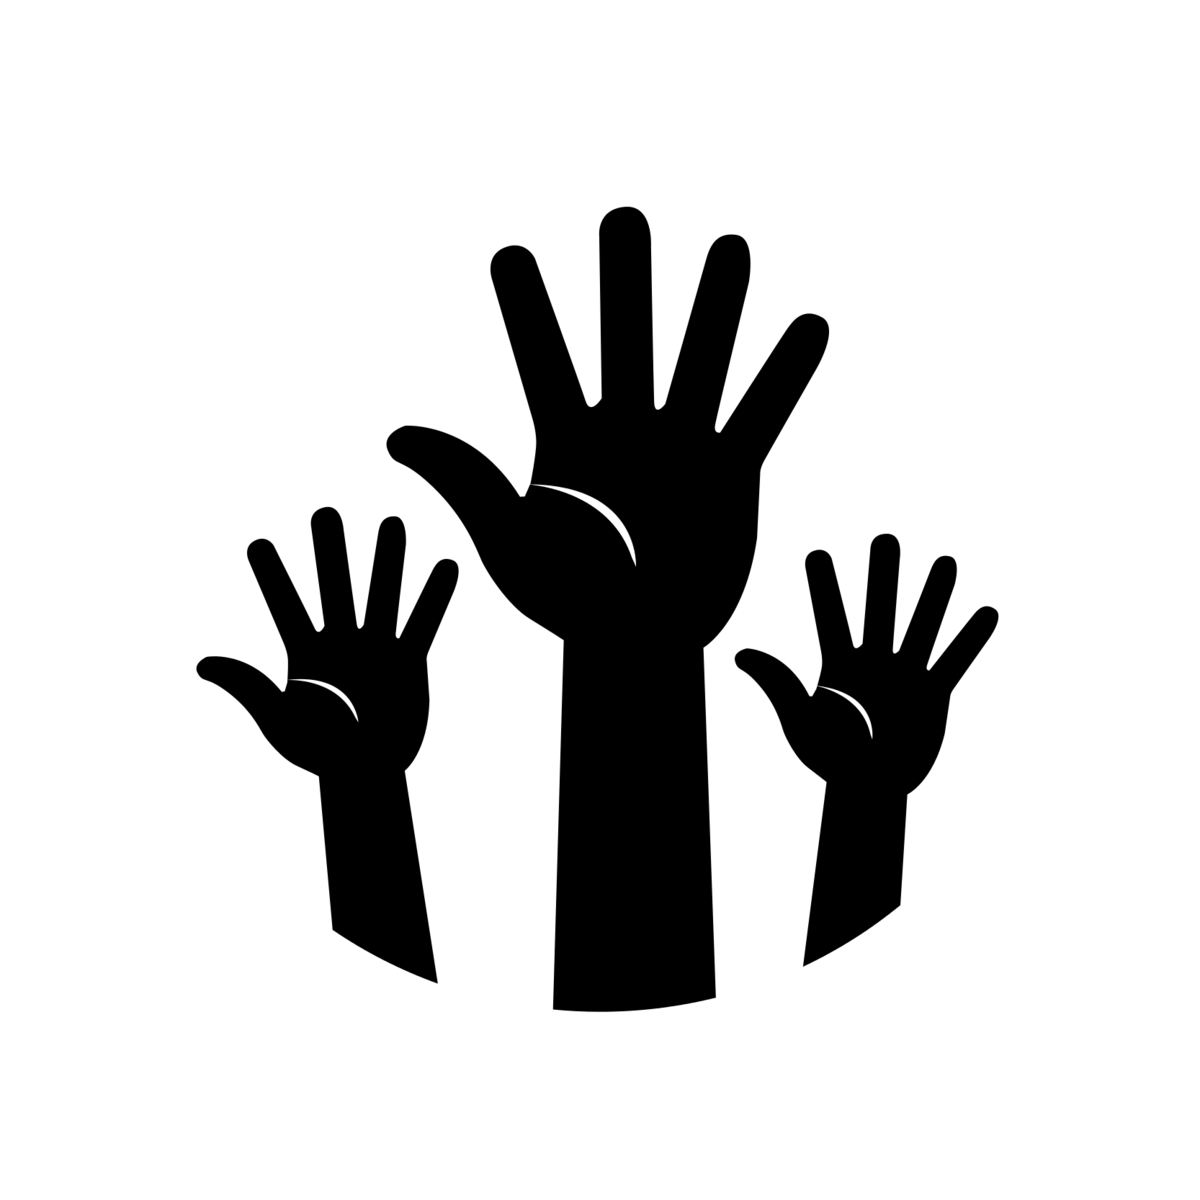
\includegraphics[height=1.5em]{images/hands}}
\newcommand{\transpose}[0]{{\textrm{\tiny{\sf{T}}}}}
\newcommand{\norm}{{\mathcal{N}}}
\newcommand{\cutoff}[0]{\kappa}
\newcommand{\instD}[0]{\dataset}
\newcommand{\insts}[0]{\mathcal{I}}
\newcommand{\inst}[0]{i}
\newcommand{\instI}[1]{i^{(#1)}}

% Iteration specific instance of variable/function/anything
% Introduced in the BO section, but moved up here to make it available within other macros
\newcommand{\iter}[2][\bocount]{{#2}^{(#1)}}

%--------HPO parameter macros-----------

% Parameter Configuration Space
\newcommand{\pcs}[0]{\pmb{\Lambda}}

% ???
\newcommand{\bx}[0]{\conf}

% Parameter Configuration
\newcommand{\conf}[0]{\pmb{\lambda}}

% Final Configuration
\newcommand{\finconf}[0]{\pmb{\hat{\lambda}}}

% Configuration corresponding to a given iteration -- better use \iter!
\newcommand{\confI}[1]{{\conf}^{(#1)}}

% Default Configuration
\newcommand{\defconf}[0]{{\conf}_{\text{def}}}

% Incumbent Configuration
\newcommand{\incumbent}[1][\bocount]{\iter[#1]{\finconf}}

% Optimal Configuration
\newcommand{\optconf}[0]{{\conf}^*}

% Configuration Space
\newcommand{\confs}[0]{\pcs}

%----------------------------------------

%\newcommand{\vlambda}[0]{\bm{\lambda}}
%\newcommand{\vLambda}[0]{\bm{\Lambda}}
\newcommand{\dataset}[0]{\mathcal{D}}
\newcommand{\datasets}[0]{\mathbf{D}}
\newcommand{\loss}[0]{L}
\newcommand{\risk}{\mathcal{R}}
\newcommand{\riske}{\mathcal{R}_{\text{emp}}}
\newcommand{\cost}[0]{c}
\newcommand{\costI}[1]{c^{(#1)}}

% Gaussian Process
\newcommand{\gp}{\mathcal{G}}
% Family of Objective Functions
\newcommand{\objF}{F}

%---------------BO Macros------------------

% BO loop counter
\newcommand{\bocount}{t}
% BO loop counter max, the counter runs from 1 to this value
\newcommand{\bobudget}{T}
% BO loop observation
\newcommand{\obs}[1][\conf]{\cost({#1})}
% BO loop observation space
\newcommand{\obsspace}{\mathcal{Y}}
% BO loop next observation
\newcommand{\bonextobs}{\obs[\iter{\conf}]}
% Acquisition Function, no args
\newcommand{\acq}{u}
% Standard Normal PDF
\newcommand{\pdf}{\phi}
% Standard Normal CDF
\newcommand{\cdf}{\Phi}
% Mean
\newcommand{\mean}{\mu}
% Standard Deviation
\newcommand{\stddev}{\sigma}
% Variance
\newcommand{\variance}{\sigma^2}
% Noise
\newcommand{\noise}{\nu}
% BO loop next selected sample
\newcommand{\bonextsample}{\confI{\bocount}}

% Single hyperparameter
\newcommand{\hyperparam}{\lambda}

% Single hyperparameter within a hyperparameter configuration
\newcommand{\hyperparami}[1][i]{{\hyperparam}_#1}

% Full definition of final configuration
\newcommand{\finconffull}{\incumbent[\bobudget]}

% Dataset
\newcommand{\datasetHPO}{{\dataset}_{HPO}}

% Dataset definition
\newcommand{\datasetHPOdef}{{\langle \bonextsample,\,\bonextobs \rangle}_{\bocount=1}^{\bobudget}}

% Double Display Fraction, forces large displays for everything in numerator and denominator
\newcommand\ddfrac[2]{\frac{\displaystyle #1}{\displaystyle #2}}

% Conditional Probability "Given That" Relation, source:https://tex.stackexchange.com/a/141685/205886
\newcommand\given[1][]{\:#1\vert\:}

% Expectation as a math operator
\DeclareMathOperator*{\E}{\mathbb{E}}

% Citation 
\newcommand{\source}[1]{
    \begin{flushright}
    	Source: \lit{#1}
    \end{flushright}
}
%-------------------------------------------

%Real numbers set
\newcommand{\realnum}{\mathbb{R}}
%Configuration space - do not use
%\newcommand{\configspace}{\Theta}
%Instances - do not use
%\newcommand{\instances}{\mathcal{I}}
%Expected value
\newcommand{\expectation}{\mathbb{E}}
%Kernel
\newcommand{\kernel}{\kappa}
%Constraint function
\newcommand{\constraintf}{c}
%Normal distribution
\newcommand{\normaldist}{\mathcal{N}}

% \renewcommand{\vec}[1]{\mathbf{#1}}
\newcommand{\hist}[0]{\dataset_{\text{Hist}}}
\newcommand{\param}[0]{p}
\newcommand{\algo}[0]{\mathcal{A}}
\newcommand{\algos}[0]{\mathbf{A}}
%\newcommand{\nn}[0]{N}
\newcommand{\feats}[0]{\mathcal{X}_{\text{meta}}}
\newcommand{\feat}[0]{\x_{\text{meta}}}
%\newcommand{\cluster}[0]{\vec{h}}
%\newcommand{\clusters}[0]{\vec{H}}
\newcommand{\perf}[0]{\mathbb{R}}
%\newcommand{\surro}[0]{\mathcal{S}}
\newcommand{\surro}[0]{\hat{\cost}}
\newcommand{\func}[0]{f}
\newcommand{\epm}[0]{\surro}
\newcommand{\portfolio}[0]{\mathbf{P}}
\newcommand{\schedule}[0]{\mathcal{S}}

% Machine Learning
\newcommand{\mdata}[0]{\dataset_{\text{meta}}}
\newcommand{\datasettrain}[0]{\dataset_{\text{train}}}
\newcommand{\datasetval}[0]{\dataset_{\text{val}}}
\newcommand{\datasettest}[0]{\dataset_{\text{test}}}
\newcommand{\x}[0]{\mathbf{x}}
\newcommand{\y}[0]{y}
\newcommand{\xI}[1]{\mathbf{x}^{(#1)}}
\newcommand{\yI}[1]{y^{(#1)}}
\newcommand{\fx}{f(\mathbf{x})}  % f(x), continuous prediction function
\newcommand{\Hspace}{\mathcal{H}} % hypothesis space where f is from
\newcommand{\fh}{\hat{f}}       % f hat, estimated prediction function

% Deep Learning
\newcommand{\weights}[0]{\theta}
\newcommand{\metaweights}[0]{\phi}


% reinforcement learning
\newcommand{\policies}[0]{\mathbf{\Pi}}
\newcommand{\policy}[0]{\pi}
\newcommand{\actionRL}[0]{a}
\newcommand{\stateRL}[0]{s}
\newcommand{\statesRL}[0]{\mathcal{S}}
\newcommand{\rewardRL}[0]{r}
\newcommand{\rewardfuncRL}[0]{\mathcal{R}}

\RestyleAlgo{algoruled}
\DontPrintSemicolon
\LinesNumbered
\SetAlgoVlined
\SetFuncSty{textsc}

\SetKwInOut{Input}{Input}
\SetKwInOut{Output}{Output}
\SetKw{Return}{return}

%\newcommand{\changed}[1]{{\color{red}#1}}

%\newcommand{\citeN}[1]{\citeauthor{#1}~(\citeyear{#1})}

\renewcommand{\vec}[1]{\mathbf{#1}}
\DeclareMathOperator*{\argmin}{arg\,min}
\DeclareMathOperator*{\argmax}{arg\,max}

%\newcommand{\aqme}{\textit{AQME}}
%\newcommand{\aslib}{\textit{ASlib}}
%\newcommand{\llama}{\textit{LLAMA}}
%\newcommand{\satzilla}{\textit{SATzilla}}
%\newcommand{\satzillaY}[1]{\textit{SATzilla'{#1}}}
%\newcommand{\snnap}{\textit{SNNAP}}
%\newcommand{\claspfolioTwo}{\textit{claspfolio~2}}
%\newcommand{\flexfolio}{\textit{FlexFolio}}
%\newcommand{\claspfolioOne}{\textit{claspfolio~1}}
%\newcommand{\isac}{\textit{ISAC}}
%\newcommand{\eisac}{\textit{EISAC}}
%\newcommand{\sss}{\textit{3S}}
%\newcommand{\sunny}{\textit{Sunny}}
%\newcommand{\ssspar}{\textit{3Spar}}
%\newcommand{\cshc}{\textit{CSHC}}
%\newcommand{\cshcpar}{\textit{CSHCpar}}
%\newcommand{\measp}{\textit{ME-ASP}}
%\newcommand{\aspeed}{\textit{aspeed}}
%\newcommand{\autofolio}{\textit{AutoFolio}}
%\newcommand{\cedalion}{\textit{Cedalion}}
\newcommand{\fanova}{\textit{fANOVA}}
\newcommand{\sbs}{\textit{SB}}
\newcommand{\oracle}{\textit{VBS}}

% like approaches
\newcommand{\claspfoliolike}[1]{\texttt{claspfolio-#1-like}}
\newcommand{\satzillalike}[1]{\texttt{SATzilla'#1-like}}
\newcommand{\isaclike}{\texttt{ISAC-like}}
\newcommand{\ssslike}{\texttt{3S-like}}
\newcommand{\measplike}{\texttt{ME-ASP-like}}

\newcommand{\irace}{\textit{I/F-race}}
\newcommand{\gga}{\textit{GGA}}
\newcommand{\smac}{\textit{SMAC}}
\newcommand{\paramils}{\textit{ParamILS}}
\newcommand{\spearmint}{\textit{Spearmint}}
\newcommand{\tpe}{\textit{TPE}}


\usepackage{pifont}
\newcommand{\itarrow}{\mbox{\Pisymbol{pzd}{229}}}
\newcommand{\ithook}{\mbox{\Pisymbol{pzd}{52}}}
\newcommand{\itcross}{\mbox{\Pisymbol{pzd}{56}}}
\newcommand{\ithand}{\mbox{\raisebox{-1pt}{\Pisymbol{pzd}{43}}}}

%\DeclareMathOperator*{\argmax}{arg\,max}

\newcommand{\ie}{{\it{}i.e.\/}}
\newcommand{\eg}{{\it{}e.g.\/}}
\newcommand{\cf}{{\it{}cf.\/}}
\newcommand{\wrt}{\mbox{w.r.t.}}
\newcommand{\vs}{{\it{}vs\/}}
\newcommand{\vsp}{{\it{}vs\/}}
\newcommand{\etc}{{\copyedit{etc.}}}
\newcommand{\etal}{{\it{}et al.\/}}

\newcommand{\pscProc}{{\bf procedure}}
\newcommand{\pscBegin}{{\bf begin}}
\newcommand{\pscEnd}{{\bf end}}
\newcommand{\pscEndIf}{{\bf endif}}
\newcommand{\pscFor}{{\bf for}}
\newcommand{\pscEach}{{\bf each}}
\newcommand{\pscThen}{{\bf then}}
\newcommand{\pscElse}{{\bf else}}
\newcommand{\pscWhile}{{\bf while}}
\newcommand{\pscIf}{{\bf if}}
\newcommand{\pscRepeat}{{\bf repeat}}
\newcommand{\pscUntil}{{\bf until}}
\newcommand{\pscWithProb}{{\bf with probability}}
\newcommand{\pscOtherwise}{{\bf otherwise}}
\newcommand{\pscDo}{{\bf do}}
\newcommand{\pscTo}{{\bf to}}
\newcommand{\pscOr}{{\bf or}}
\newcommand{\pscAnd}{{\bf and}}
\newcommand{\pscNot}{{\bf not}}
\newcommand{\pscFalse}{{\bf false}}
\newcommand{\pscEachElOf}{{\bf each element of}}
\newcommand{\pscReturn}{{\bf return}}

%\newcommand{\param}[1]{{\sl{}#1}}
\newcommand{\var}[1]{{\it{}#1}}
\newcommand{\cond}[1]{{\sf{}#1}}
%\newcommand{\state}[1]{{\sf{}#1}}
%\newcommand{\func}[1]{{\sl{}#1}}
\newcommand{\set}[1]{{\Bbb #1}}
%\newcommand{\inst}[1]{{\tt{}#1}}
\newcommand{\myurl}[1]{{\small\sf #1}}

\newcommand{\Nats}{{\Bbb N}}
\newcommand{\Reals}{{\Bbb R}}
\newcommand{\extset}[2]{\{#1 \; | \; #2\}}

\newcommand{\vbar}{$\,\;|$\hspace*{-1em}\raisebox{-0.3mm}{$\,\;\;|$}}
\newcommand{\vendbar}{\raisebox{+0.4mm}{$\,\;|$}}
\newcommand{\vend}{$\,\:\lfloor$}


\newcommand{\goleft}[2][.7]{\parbox[t]{#1\linewidth}{\strut\raggedright #2\strut}}
\newcommand{\rightimage}[2][.3]{\mbox{}\hfill\raisebox{1em-\height}[0pt][0pt]{\includegraphics[width=#1\linewidth]{#2}}\vspace*{-\baselineskip}}





\newcommand{\inducer}{\mathcal{I}}
\newcommand{\R}{\mathds{R}}

%The following might look confusing but allows us to switch the notation of the optimization problem independently from the notation of the hyper parameter optimization
\newcommand{\xx}{\conf} %x of the optimizer
\newcommand{\xxi}[1][i]{\conf_{#1}} %i-th component of xx (not confuse with i-th individual)
\newcommand{\XX}{\pcs} %search space / domain of f
\newcommand{\f}{\cost} %objective function

\newenvironment{blocki}[1] % itemize block
{
 \begin{block}{#1}\begin{itemize}
}
{
\end{itemize}\end{block}
}

\title[AutoML: Hyperparameter Optimization]{AutoML: Hyperparameter Optimization}
%\subtitle{Overview for this Week} %To be defined in source!
%TODO: change authors!
\author[Marius Lindauer]{\underline{Bernd Bischl} \and Frank Hutter \and Lars Kotthoff\newline \and Marius Lindauer \and Joaquin Vanschoren}
\institute{}
\date{}


\usepackage{ulem}
\usepackage{pifont}

\subtitle{Wrap Up}


\begin{document}

\maketitle


%----------------------------------------------------------------------
%----------------------------------------------------------------------

\begin{frame}{From HPO to AutoML}
  So far we covered
  \begin{itemize}
    \item Mechanisms to select promising ML Algorithms for a Dataset (Algorithm Selection)
    \item HPO as Black-Box optimization
    \begin{itemize}
      \item Grid- and Random Search, Evolutionary Algorithms, Bayesian Optimization
    \end{itemize}
    \item HPO as a Grey-Box-Problem
    \begin{itemize}
      \item Hyperband, BOHB
    \end{itemize}
    \item Optimizing Neural Network Architectures (NAS)
    \begin{itemize}
      \item One-Shot approaches, DART
    \end{itemize}
    \item Dynamic Algorithm Configuration (Learning to Learn)
    \begin{itemize}
      \item Adapt hyperparameter during training. 
    \end{itemize}
  \end{itemize}  
\end{frame}

\begin{frame}{From HPO to AutoML}
    \begin{center}
      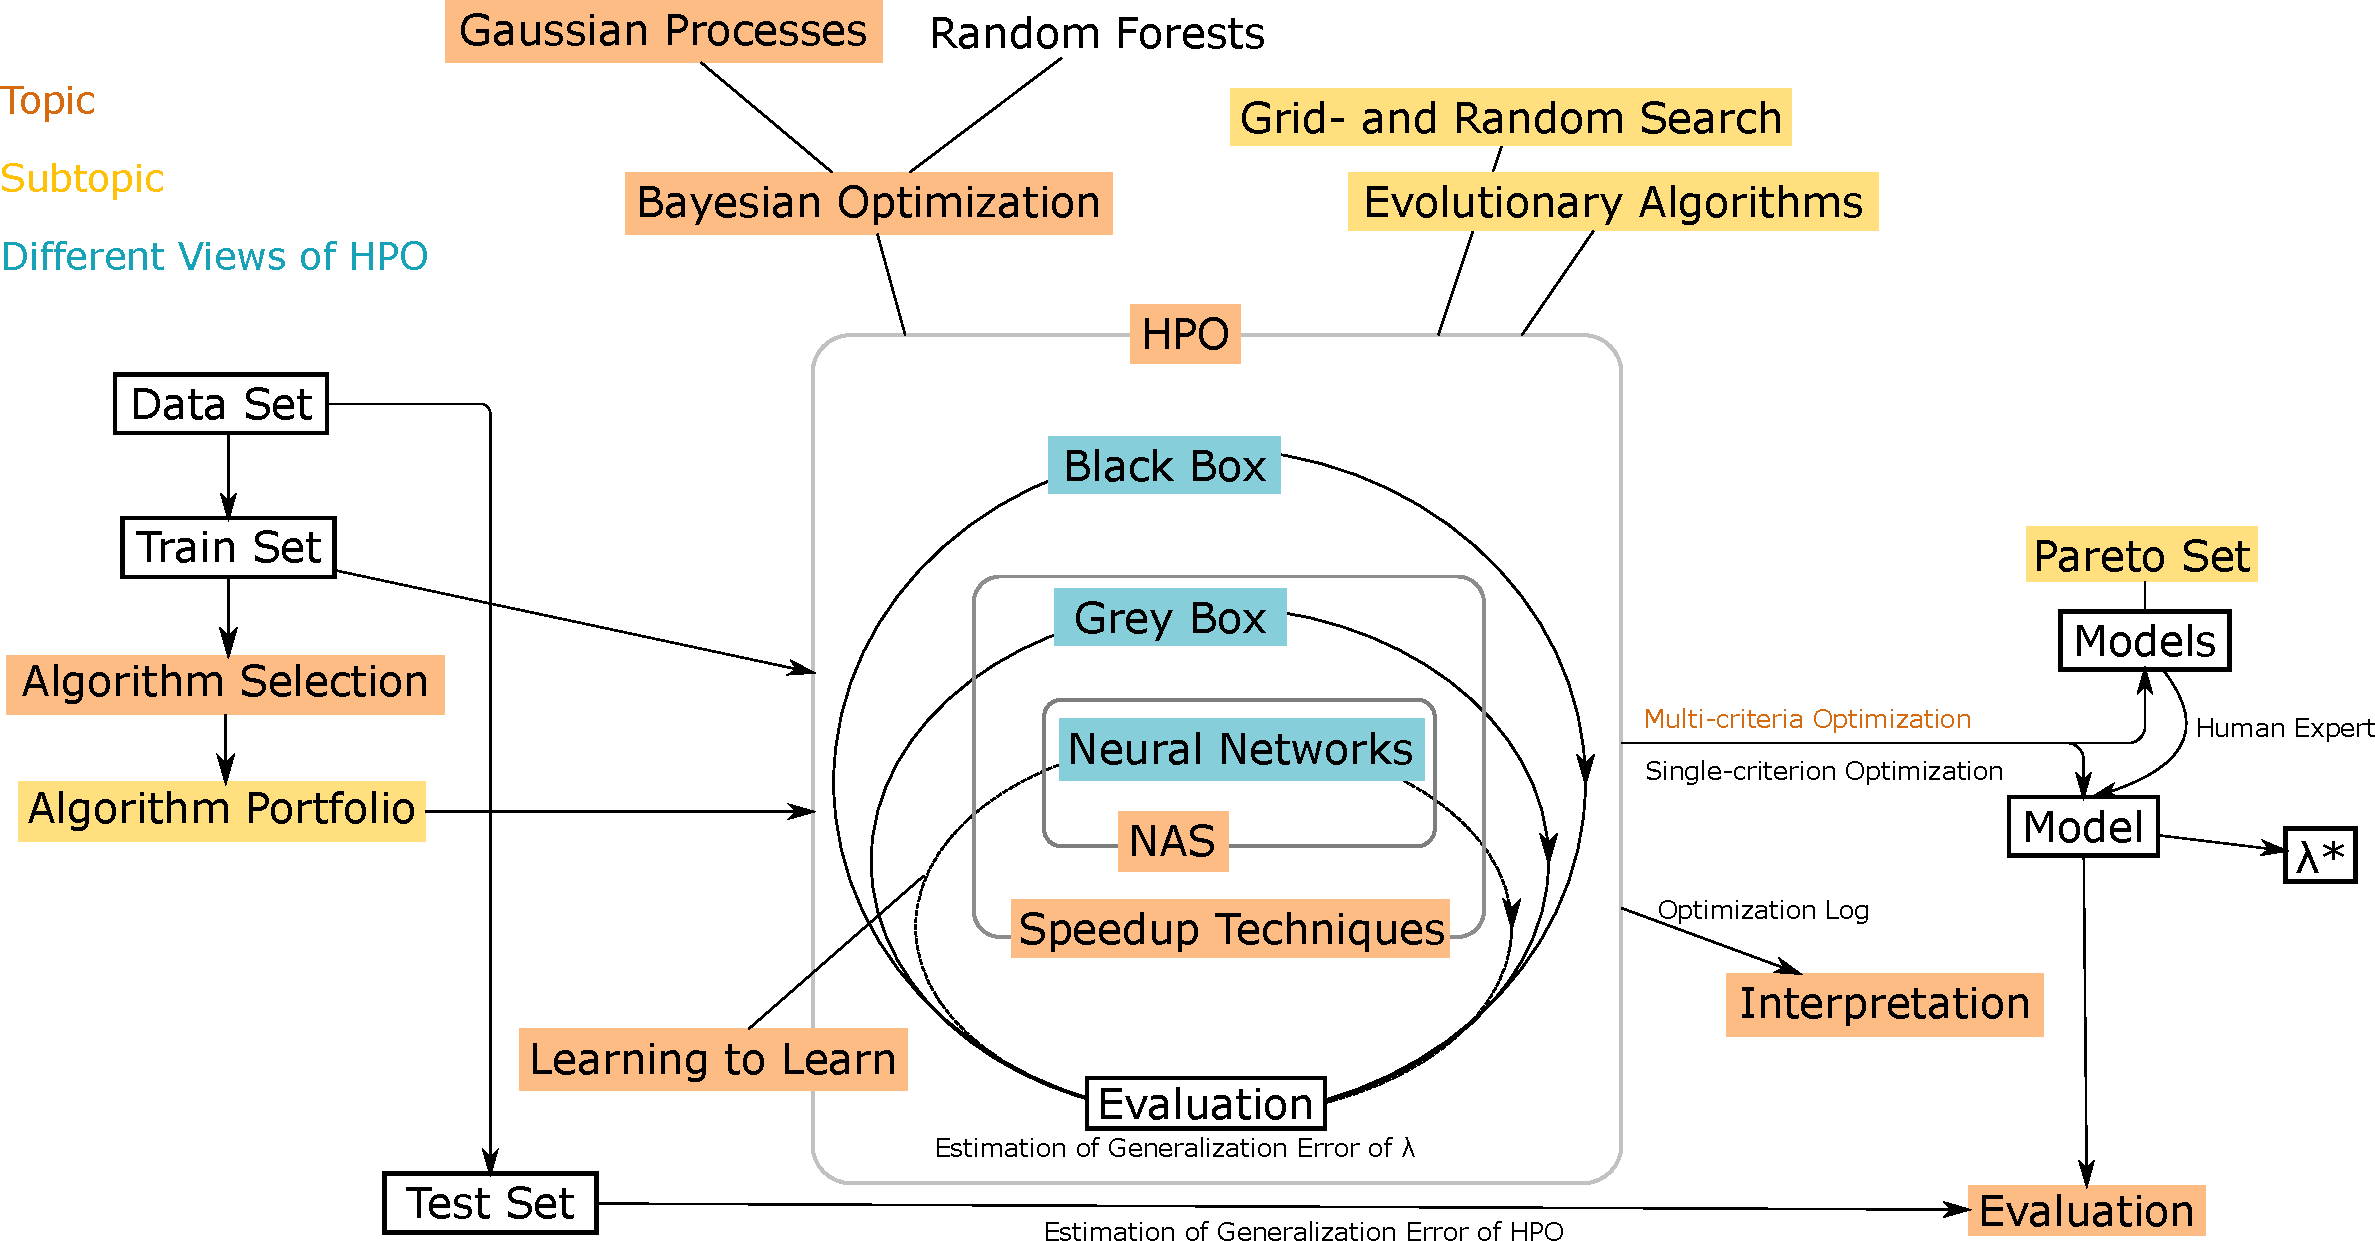
\includegraphics[width = 0.9\linewidth]{images/drawing.pdf}  
    \end{center}
\end{frame}

\section{The Missing Building Blocks}

\begin{frame}{What is missing?}
  \begin{columns}
    \begin{column}{0.5\textwidth}
        What do I need to know as an AutoML user?
        \begin{itemize}
          \item \sout{Nothing, because it is automatic.}
          \item Understand limitations of the framework you are using.
          \item Know how to interpret the results.
          \item Possibly, how to preprocess the data.
        \end{itemize}

        \vspace{1em}

        What do I need to implement an AutoML framework?
        \begin{itemize}
          \item HPO Algorithm
          \item ML Algorithm (= Design Space)
          \item Resampling
          \item (Preprocessing)
        \end{itemize}
    \end{column}%
    \begin{column}{0.5\textwidth}
      \begin{center}
        Academic view:
        \scalebox{0.45}{
          \begin{tikzpicture}[node distance=4cm, thick]
	\node (function) [data] {Cost $\cost$};
	\node (budget) [data, below of=function, node distance=1cm] {Budgets};
	\node (space) [data, below of=budgets, node distance=1cm] {Design Space $\pcs$};
  \node (resampling) [data, below of=space, node distance=1cm] {Resampling};
	
	\node (hb) [activity, right of=space, node distance=6cm, yshift=-.5cm] {ML System};
	\node (kde) [activity, above of=hb, node distance=2cm] {AutoML Optimizer};
	
	\draw[myarrow] ($(kde.south)+(-0.3,0.0)$) -- ++(0.0,-0.6) node[left] {$\conf \in \pcs$} -- ($(hb.north)+(-0.3,+0.0)$);
	\draw[myarrow] ($(hb.north)+(0.3,+0.0)$) -- ++(0.0,0.6) node[right] {$\cost(\conf)$} -- ($(kde.south)+(0.3,0.0)$);
	
	\draw[myarrow] (function.east) -- ($(kde.west)+(-0.3,0.5)$);
	\draw[myarrow] (budgets.east) -- ($(kde.west)+(-0.3,-0.5)$);
	\draw[myarrow] (space.east) -- ($(kde.west)+(-0.3,-1.5)$);
  \draw[myarrow] (resampling.east) -- ($(kde.west)+(-0.3,-2.5)$);
	
	\node (perf) [activity, right of=kde, node distance=6.3cm] {Performance Analysis};
	\node (budget) [activity, below of=perf, node distance=1.2cm] {Incumbent Analysis};
	\node (imp) [activity, below of=budget, node distance=1cm] {Space Analysis};
	
	\draw[myarrow] ($(kde.east)+(0.3,-1.)$) -- node[above] {$\langle \conf^{(i)}, \cost(\confI{i}) \rangle_i$} ($(perf.west)+(-0.3,-1.)$);
	\draw[myarrow] ($(kde.east)+(0.3,-1.)$) -- node[below] {$\incumbent$} ($(perf.west)+(-0.3,-1.)$);
	
	\begin{pgfonlayer}{background}
	
	% Configuration Process
	\path (kde -| kde.west)+(-0.25,0.85) node (resUL) {};
	\path (hb.east |- hb.south)+(0.25,-0.5) node(resBR) {};
	\path [rounded corners, draw=black!60, dashed] (resUL) rectangle (resBR);
	\path (hb.east |- hb.south)+(-.5,-.1) node [text=black!60] {};
	
	\path (perf -| perf.west)+(-0.25,0.85) node (resUL) {};
	\path (imp.east |- imp.south)+(0.25,-0.5) node(resBR) {};
	\path [rounded corners, draw=black!60, dashed] (resUL) rectangle (resBR);
	\path (imp.east |- imp.south)+(-.5,-.2) node [text=black!60] {};
	
	\end{pgfonlayer}

\end{tikzpicture}
        }

        \vspace{1em}

        Practitioners view:
        \scalebox{0.45}{
          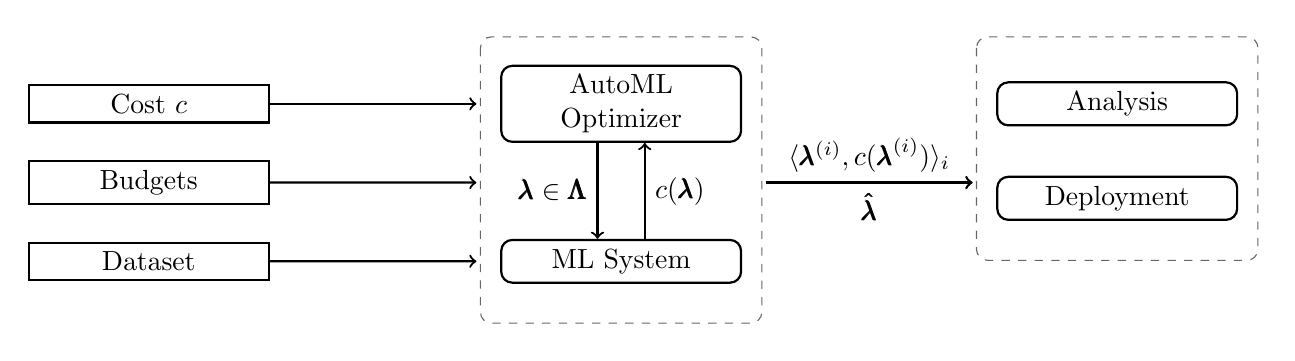
\begin{tikzpicture}[node distance=4cm, thick]
  \node (function) [data] {Cost $\cost$};
  \node (budgets) [data, below of=function, node distance=1cm] {Budgets};
  \node (dataset) [data, below of=budgets, node distance=1cm] {Dataset};
  
  \node (hb) [activity, right of=dataset, node distance=6cm, yshift=-0.0cm] {ML System};
  \node (kde) [activity, above of=hb, node distance=2cm] {AutoML Optimizer};
  
  \draw[myarrow] ($(kde.south)+(-0.3,0.0)$) -- ++(0.0,-0.6) node[left] {$\conf \in \pcs$} -- ($(hb.north)+(-0.3,+0.0)$);
  \draw[myarrow] ($(hb.north)+(0.3,+0.0)$) -- ++(0.0,0.6) node[right] {$\cost(\conf)$} -- ($(kde.south)+(0.3,0.0)$);
  
  \draw[myarrow] (function.east) -- ($(kde.west)+(-0.3,0.0)$);
  \draw[myarrow] (budgets.east) -- ($(kde.west)+(-0.3,-1.)$);
  \draw[myarrow] (dataset.east) -- ($(kde.west)+(-0.3,-2.)$);
  
  \node (perf) [activity, right of=kde, node distance=6.3cm] {Analysis};
  \node (budget) [activity, below of=perf, node distance=1.2cm] {Deployment};
  %\node (imp) [activity, below of=budget, node distance=1cm] {Space Analysis};
  
  \draw[myarrow] ($(kde.east)+(0.3,-1.)$) -- node[above] {$\langle \conf^{(i)}, \cost(\confI{i}) \rangle_i$} ($(perf.west)+(-0.3,-1.)$);
  \draw[myarrow] ($(kde.east)+(0.3,-1.)$) -- node[below] {$\finconf$} ($(perf.west)+(-0.3,-1.)$);
  
  \begin{pgfonlayer}{background}
  
  % Configuration Process
  \path (kde -| kde.west)+(-0.25,0.85) node (resUL) {};
  \path (hb.east |- hb.south)+(0.25,-0.5) node(resBR) {};
  \path [rounded corners, draw=black!60, dashed] (resUL) rectangle (resBR);
  \path (hb.east |- hb.south)+(-.5,-.3) node [text=black!60] {};
  
  \path (perf -| perf.west)+(-0.25,0.85) node (resUL) {};
  \path (budget.east |- budget.south)+(0.25,-0.5) node(resBR) {};
  \path [rounded corners, draw=black!60, dashed] (resUL) rectangle (resBR);
  \path (budget.east |- budget.south)+(-.5,-.3) node [text=black!60] {};
  
  \end{pgfonlayer}

\end{tikzpicture}
        }
      \end{center}
    \end{column}
  \end{columns}
\end{frame}

\begin{frame}{Automate HPO}

  \begin{columns}
    \begin{column}{0.59\textwidth}

      For AutoML the user only supplies \ldots
      \begin{itemize}
        \item dataset,
        \item performance measure and
        \item possibly a time limit.
      \end{itemize}

      To do HPO we need to \ldots
      \begin{itemize}
        \item preprocessing manually,
        \item decide on an optimization algorithm,
        \item an ML algorithm (to generate Inducer $\inducer$),
        \item a search space $\pcs$ and
        \item a resampling strategy to evaluate $\cost(\conf)$.
      \end{itemize}

      To build an AutoML System we have to make these choices automatically $\rightarrow$ Following slides.

    \end{column}%
    \begin{column}{0.4\textwidth}
      \begin{center}
        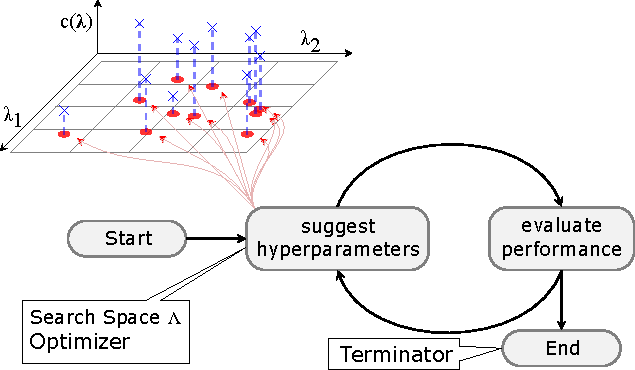
\includegraphics[width = \linewidth]{images/tuning.pdf}    
      \end{center}
    \end{column}
  \end{columns}

\end{frame}

\begin{frame}{Choice of Learning Algorithm}
  \begin{itemize}
    \item A good AutoML System should consider more than one learning algorithm. More on that later.
    \item A plethora of learning algorithm exists.
    \item Studies\footnote{\href{https://dl.acm.org/doi/10.5555/2627435.2697065}{Delgado et al., JMLR 2014}} and experience have shown that one representative of these categories usually reaches best performance (on tabular data):
    \begin{itemize}
      \item Penalized Regression, SVM, Gradient Boosting, Random Forests, Neural Networks
      \item (tuned) random forests only beaten on few datasets by current AutoML frameworks\footnote{\href{https://arxiv.org/abs/1907.00909}{Gijsbers et al., 2019}}.
      \item Example: Auto-Sklearn 2.0\footnote{\href{https://arxiv.org/abs/2007.04074}{Feurer et al., 2020}} uses: Extra Trees, Gradient Boosting, Passive Aggressive, Random Forest, Linear Model
    \end{itemize}
  \end{itemize}
\end{frame}

\begin{frame}{Choice of Search Space for a Learning Algorithm}
  \begin{columns}
    \begin{column}{0.6\textwidth}
    Which hyperparameters should we consider for a given learning algorithm?
    \begin{itemize}
      \item Ranges often selected based on experience
      \begin{itemize}
        \item Compare to other AutoML Frameworks: e.g.\ Auto-Sklearn 2.0~\lit{\href{https://arxiv.org/abs/2007.04074}{Feurer et al., 2020}} 
      \end{itemize}
      \item Sensitivity analysis does not exist for each learning algorithm
      \item Solution: Analysis of previous HPO runs and learn mapping $\datasets \rightarrow \mathcal{P}(\pcs)$ is risky (leaving out important ranges) and complicated.
      \item Instead: Use big search space $\pcs$ and try to predict good initial design (e.g.\ for Bayesian Optimization).
    \end{itemize}
    \end{column}%
    \begin{column}{0.4\textwidth}
      \begin{center}
        \only<1>{
          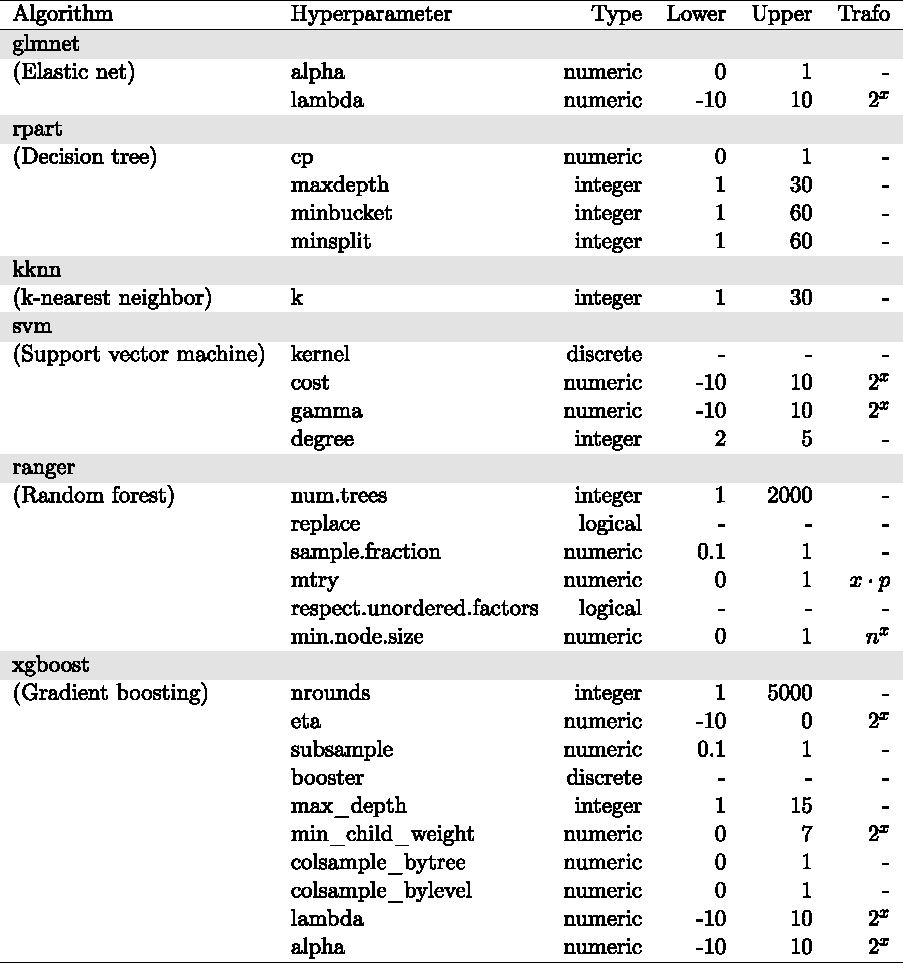
\includegraphics[width = 0.8\linewidth]{images/probst2019jmlr_tab1.pdf}
        }
        \only<2>{
          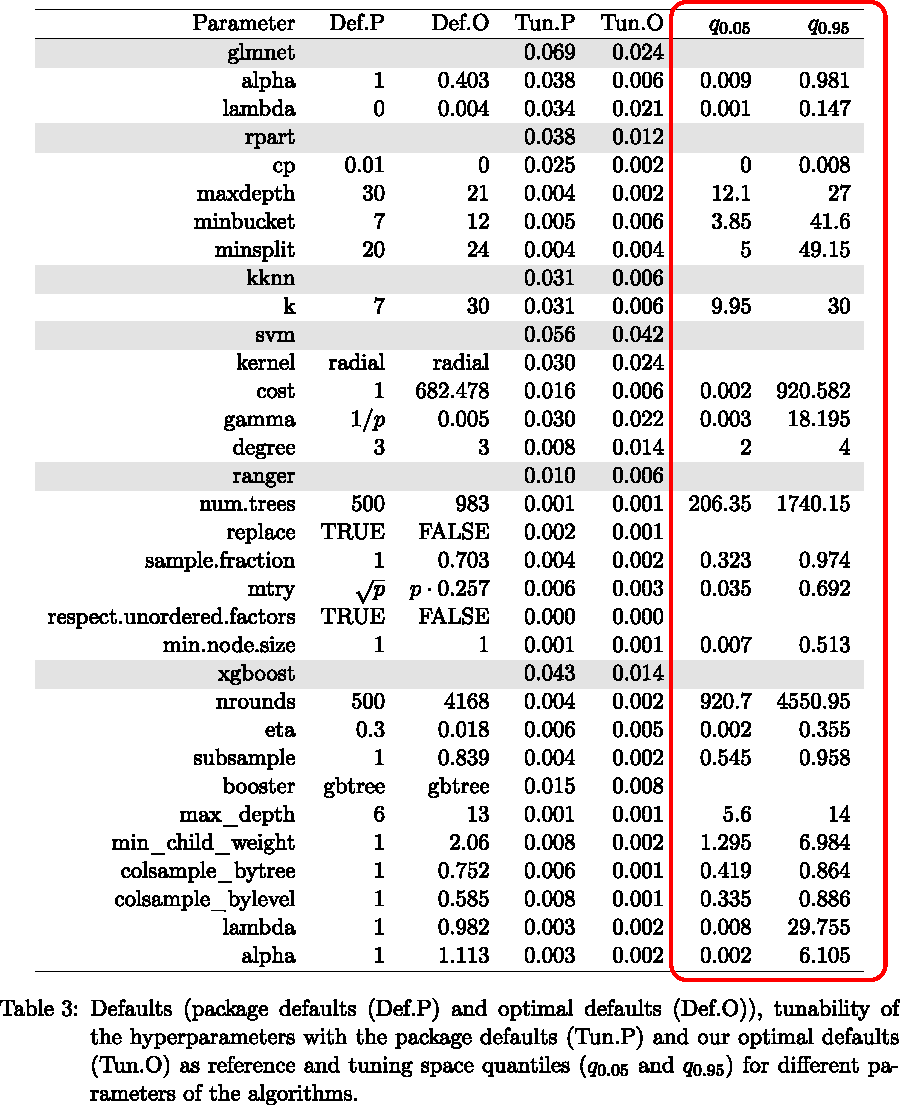
\includegraphics[width = 0.8\linewidth]{images/probst2019jmlr_tab3.pdf}   
        }

        {\tiny Taken from \href{https://www.jmlr.org/papers/volume20/18-444/18-444.pdf}{Probst et al., 2019 JMLR}.}
      \end{center}
    \end{column}
  \end{columns}
\end{frame}

\begin{frame}{Choice of Resampling Strategy}
  For the calculation of the generalization error / cost
  \begin{equation}
    \cost(\conf) = \frac{1}{R}\sum_{i = 1}^R \widehat{GE}_{\dataset_{\text{val}, i}}\left(\inducer(\dataset_{\text{train}, i}, \conf)\right)
  \end{equation}
  that defines the objective of the black-box optimization we need a resampling strategy.

  \vspace{1em}

  A heuristic to select a suitable resampling strategy may follow this rule of thumb:
    \begin{itemize}
      \item Default: 10-fold CV ($R=10$)
      \item Huge datasets: Holdout
      \item Tiny datasets: LOO
      \item For class imbalances:
      \begin{itemize}
        \item use stratification,
        \item ensure that validation split includes minority class.
      \end{itemize}
    \end{itemize}
    Or let the user decide.
\end{frame}

\begin{frame}{Choice of Optimization Algorithm}
  Choose optimization algorithm based on \ldots
  \begin{itemize}
    \item complexity of search space and
    \item estimated number of possible evaluations
  \end{itemize}

  \vspace{0.5em}

  Complex search space and many possible evaluations 
  \begin{itemize}
    \item[$\rightarrow$] Random Search, TPE, BO with RF as Surrogate
    \item[$\rightarrow$] Make use of Grey-Box Optimizers: Hyperband, BOHB
  \end{itemize}
  Simple search space and few possible Evaluations 
  \begin{itemize}
    \item[$\rightarrow$] BO with Kriging as surrogate
    \item[$\rightarrow$] Grey-Box: BOHB
  \end{itemize}
  Complex search space and few possible evaluations
  \begin{itemize}
    \item[$\rightarrow$]Use good defaults, Meta-Learning
  \end{itemize}
  Deep Neural Network Architecture Search 
  \begin{itemize}
    \item[$\rightarrow$]NAS Algorithms and possibly HPO on found architecture
  \end{itemize}

\end{frame}



\begin{frame}{Preprocessing}
  \begin{columns}
    \begin{column}{0.5\textwidth} 
      Ideal AutoML system would automatically optimize the following steps wrt.\ given cost function:
      \begin{itemize}
        \item[\ding{55}] Data cleaning
        \item[\ding{55}] Feature engineering
        \begin{itemize}
          \item Preprocessing
          \item Feature selection
          \item Feature construction  
        \end{itemize}
        \item[\ding{51}] Model training
      \end{itemize}
    We already know how to optimize the ml algorithm. How about the preprocessing steps?
    \end{column}%
    \begin{column}{0.5\textwidth}
      \begin{center}
        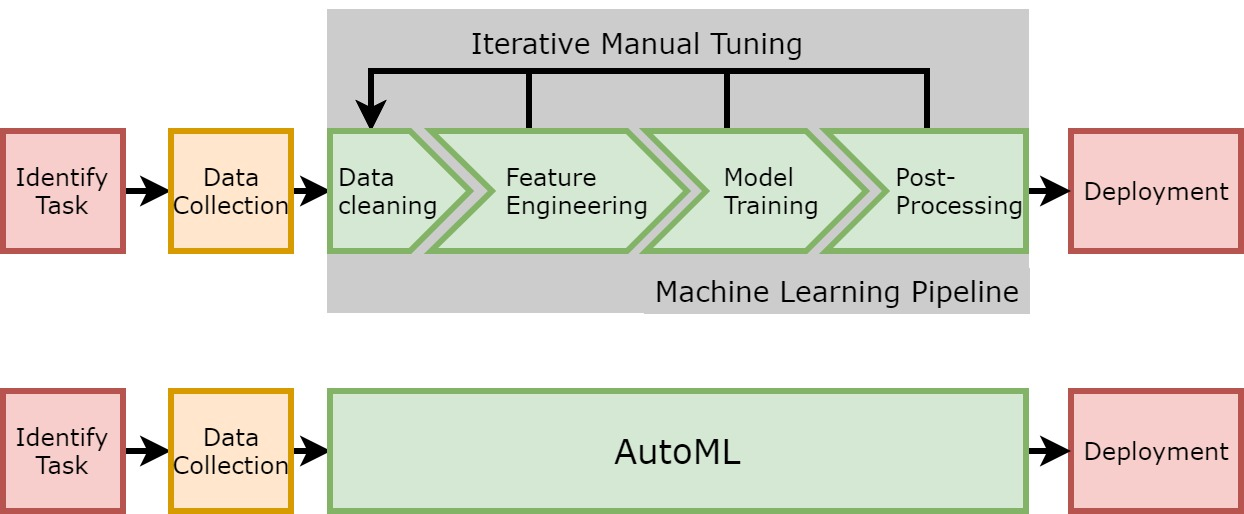
\includegraphics[width = \linewidth]{images/AutoMLPipeline.jpg}  
      \end{center}
    \end{column}
  \end{columns}
  
\end{frame}

\section{Common Preprocessing Steps}

\begin{frame}{Preprocessing not the strength of Non-commercial AutoML}
  \begin{columns}
    \begin{column}{0.6\textwidth}
      \vspace*{-1cm}
      \begin{center}
        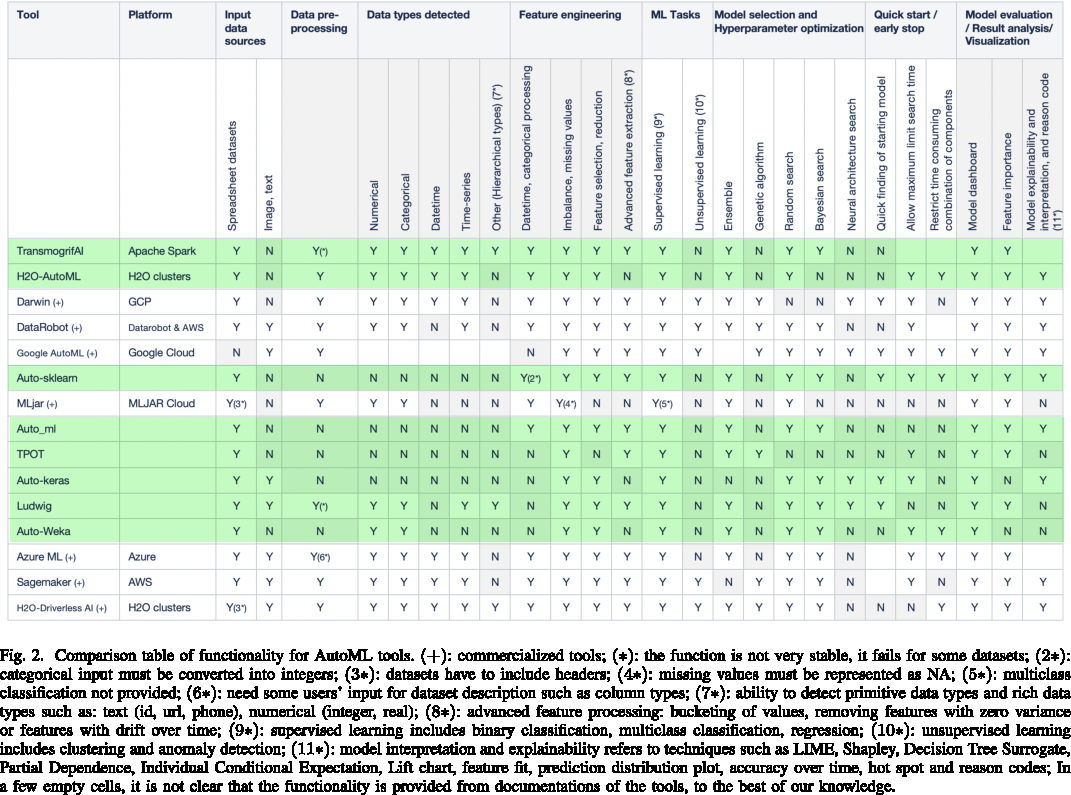
\includegraphics[width = \linewidth]{images/Truong2019Towards_fig2.pdf}
      \end{center}
    \end{column}%
    \begin{column}{0.3\textwidth}
    \small
      Taken from \href{https://doi.org/10.1109/ICTAI.2019.00209}{Truong et al., 2019 ICTAI}.
      \vspace{1em}

      Highlighted: Non-commercial AutoML Frameworks
    \end{column}
  \end{columns}
\end{frame}

\begin{frame}{Cleaning}
  Data cleaning can hardly be automatized but a few heuristics exist:
  \begin{itemize}
    \item Remove ID Columns, Columns with mostly unique values.
    \item Outlier detection (in the feature space)
    \item Detect time series or spatial data $\rightarrow$ randomized validation might be flawed.
  \end{itemize}
\end{frame}

\begin{frame}{Categorical Features: Dummy Encoding}
  % Goals:
  % \begin{itemize}
  %   \item Convert all categorical features.
  %   \item Avoid high cardinality categorical features.
  % \end{itemize}
  ML algorithm does not support categorical features + few unique values $\rightarrow$ use dummy encoding.
  \begin{center}
    \resizebox{0.3\linewidth}{!}{
    \begin{tabular}{r|l|l}
    \hline
    SalePrice & Central.Air & Bldg.Type\\
    \hline
    189900 & Y & 1Fam\\
    \hline
    195500 & Y & 1Fam\\
    \hline
    213500 & Y & TwnhsE\\
    \hline
    191500 & Y & TwnhsE\\
    \hline
    236500 & Y & TwnhsE\\
    \hline
    \end{tabular}
    } \\
    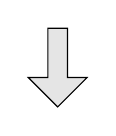
\begin{tikzpicture}
      %\useasboundingbox (-2,0);
      \node[single arrow,draw=black,fill=black!10,minimum height=1cm,shape border rotate=270] at (0,-1) {};
    \end{tikzpicture} \\
  \resizebox{0.9\linewidth}{!}{
    \begin{tabular}{r|r|r|r|r|r}
    \hline
    SalePrice & Y & Bldg.Type.2fmCon & Bldg.Type.Duplex & Bldg.Type.Twnhs & Bldg.Type.TwnhsE\\
    \hline
    189900 & 1 & 0 & 0 & 0 & 0\\
    \hline
    195500 & 1 & 0 & 0 & 0 & 0\\
    \hline
    213500 & 1 & 0 & 0 & 0 & 1\\
    \hline
    191500 & 1 & 0 & 0 & 0 & 1\\
    \hline
    236500 & 1 & 0 & 0 & 0 & 1\\
    \hline
    \end{tabular}
  }
  \end{center}
\end{frame}

\begin{frame}{Categorical Features: Target Encoding}
  Avoid high cardinality categorical features because they are problematic for all ML algorithms $\rightarrow$ use Target Encoding (also Impact Encoding).
  \begin{columns}
    \begin{column}{0.7\textwidth}


      \textbf{Goal}: Each categorical feature $\bm{x}$ should be encoded in a single numeric feature $\tilde{\bm{x}}$
      
      \vspace*{-0.5cm}  
      {\footnotesize
      \begin{align*}
      \text{Regression:} \operatorname{Impact}(x) &= \E(\bm{y} | x) - \E(\bm{y}) \\
      \text{Classification:} \operatorname{Impact}(x) &= \operatorname{logit}(P( y = \text{target} | x)) - \operatorname{logit}(P( y = \text{target}))
      \end{align*}
      }
      \vspace*{-0.5cm}  
      \begin{itemize}
        \item Needs regularization (through CV) to prevent target leakage \lit{\href{https://arxiv.org/abs/1611.09477}{Zumel et al., 2019}}
        \item Advantage: Handles unknown categorical levels on test data.
      \end{itemize}
      Alternatives: Factorization Machines, clustering feature levels, feature hashing
    \end{column}%
    \begin{column}{0.3\textwidth}
      \begin{center}
        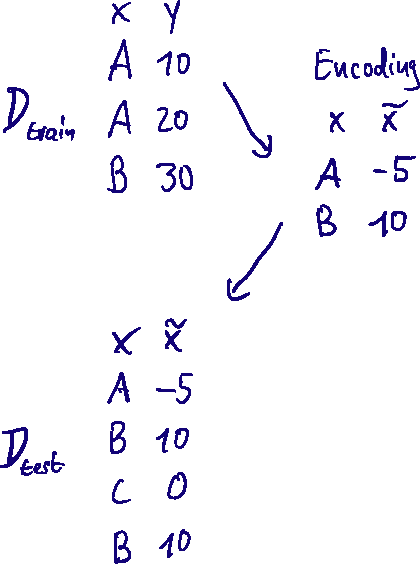
\includegraphics[width = \textwidth]{images/scetch_impact_encoding.pdf}
      \end{center}
    \end{column}
  \end{columns}
\end{frame}

\begin{frame}{Common Preprocessing Steps: Missing Values}
  Missing values:
  \begin{itemize}
    \item Additional factor column indicating missingness
    \item Replace missing values with \emph{out of range} or median/mode
    \item Advanced imputation strategies seldom advantageous (also because data mostly not missing at random)
  \end{itemize}
\end{frame}

\begin{frame}{Feature Selection}
    \begin{columns}
      \begin{column}{0.4\textwidth}
        Feature selection:
        \begin{itemize}
          \item Filter
          \item Stepwise selection methods: Needs to be applied on the whole pipeline (impractical!)
          \item Seldom increases performance but decreases computational costs $\rightarrow$ Multi-criteria optimization.
          \begin{itemize}
            \item Combined Feature Selection and HPO: \lit{\href{https://doi.org/10.1145/3377930.3389815}{Binder et al., 2020 GECCO}}
          \end{itemize}
          \item Happens indirectly in learning algorithm: random forest, lasso regression, \ldots %FIXME More examples.
        \end{itemize}
      \end{column}%
      \begin{column}{0.6\textwidth}
        \begin{center}
          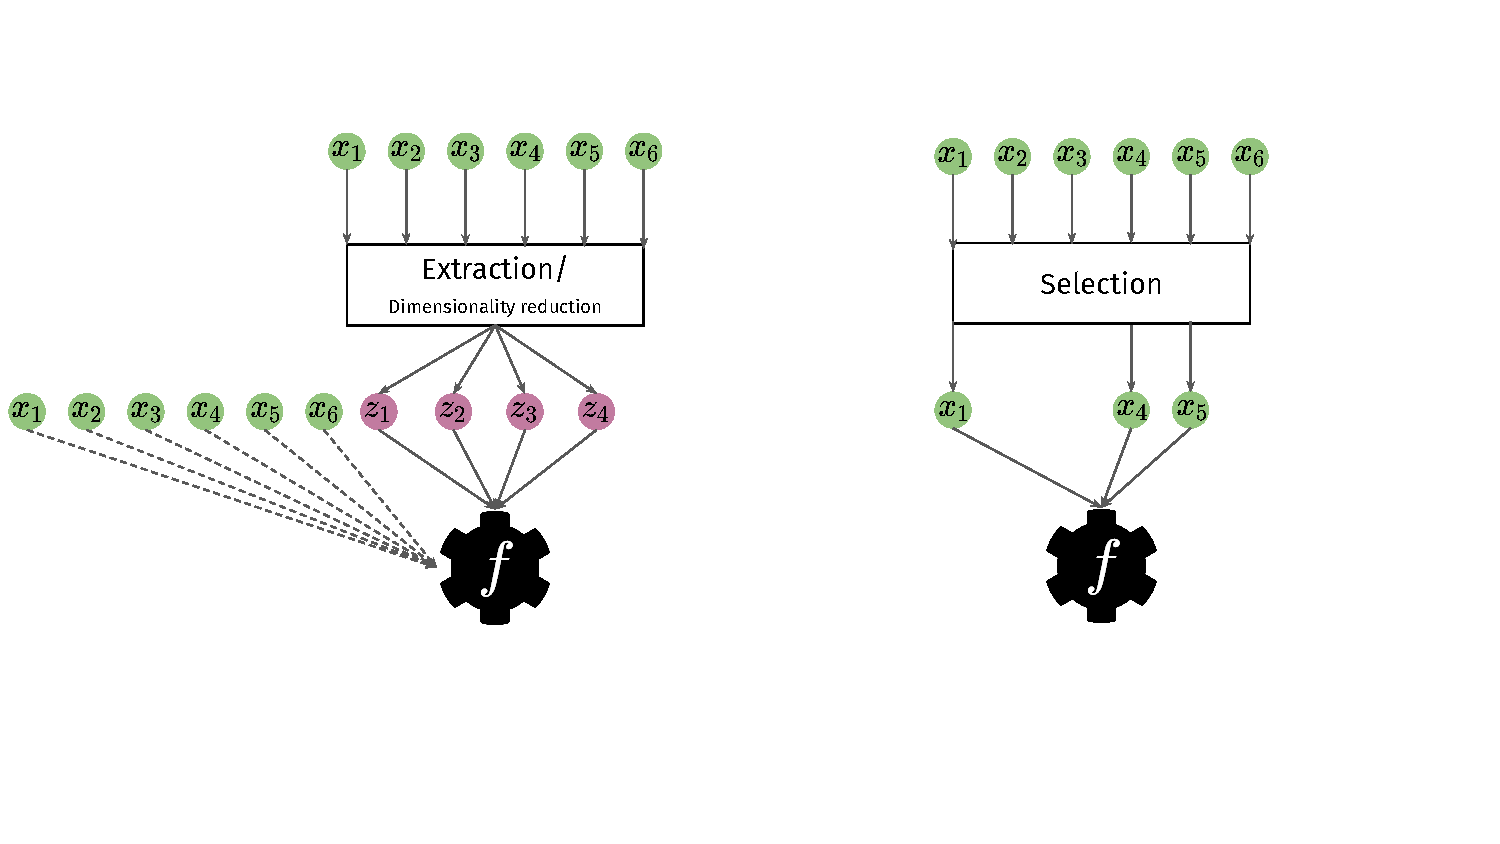
\includegraphics[width=0.35\textwidth, trim=450 100 110 60, clip]{images/feat_extr_vs_selection.pdf}%
          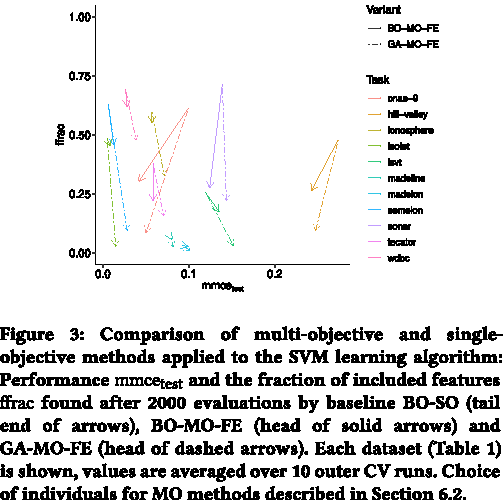
\includegraphics[width=0.55\linewidth]{images/Binder2020multiobjective_fig3.pdf}

          {\tiny \hfill Taken from \href{https://doi.org/10.1145/3377930.3389815}{Binder et al., 2020 GECCO}.}
        \end{center}
      \end{column}
    \end{columns}
    
\end{frame}

\begin{frame}{Common Feature Construction Methods}
  \begin{columns}
    \begin{column}{0.6\textwidth}
    Reduction:
    \begin{itemize}
      \item PCA, ICA, autoencoder
    \end{itemize}

    Feature extraction:
    \begin{itemize}
      \item Polynomial Features: $x_j \longrightarrow x_j, x_j^2, x_j^3, ...$
      \item Interactions: $x_j, x_k \longrightarrow x_j, x_k, x_j \cdot x_k$
    \end{itemize}

    Feature generation:
    \begin{itemize}
      \item Transform to ``circular'' features (year, month, day) \\
      e.g.\ $\tilde x_1 = sin(2\pi \cdot x /24)$ and $\tilde x_2 = cos(2\pi \cdot x /24)$
    \end{itemize}
    
    Combine with external data:
    \begin{itemize}
      \item names $\longrightarrow$ gender, ethnicity, age
      \item home address $\longrightarrow$ household income
      \item location + date $\longrightarrow$ weather
    \end{itemize}

    \end{column}%
    \begin{column}{0.4\textwidth}
      \begin{center}
        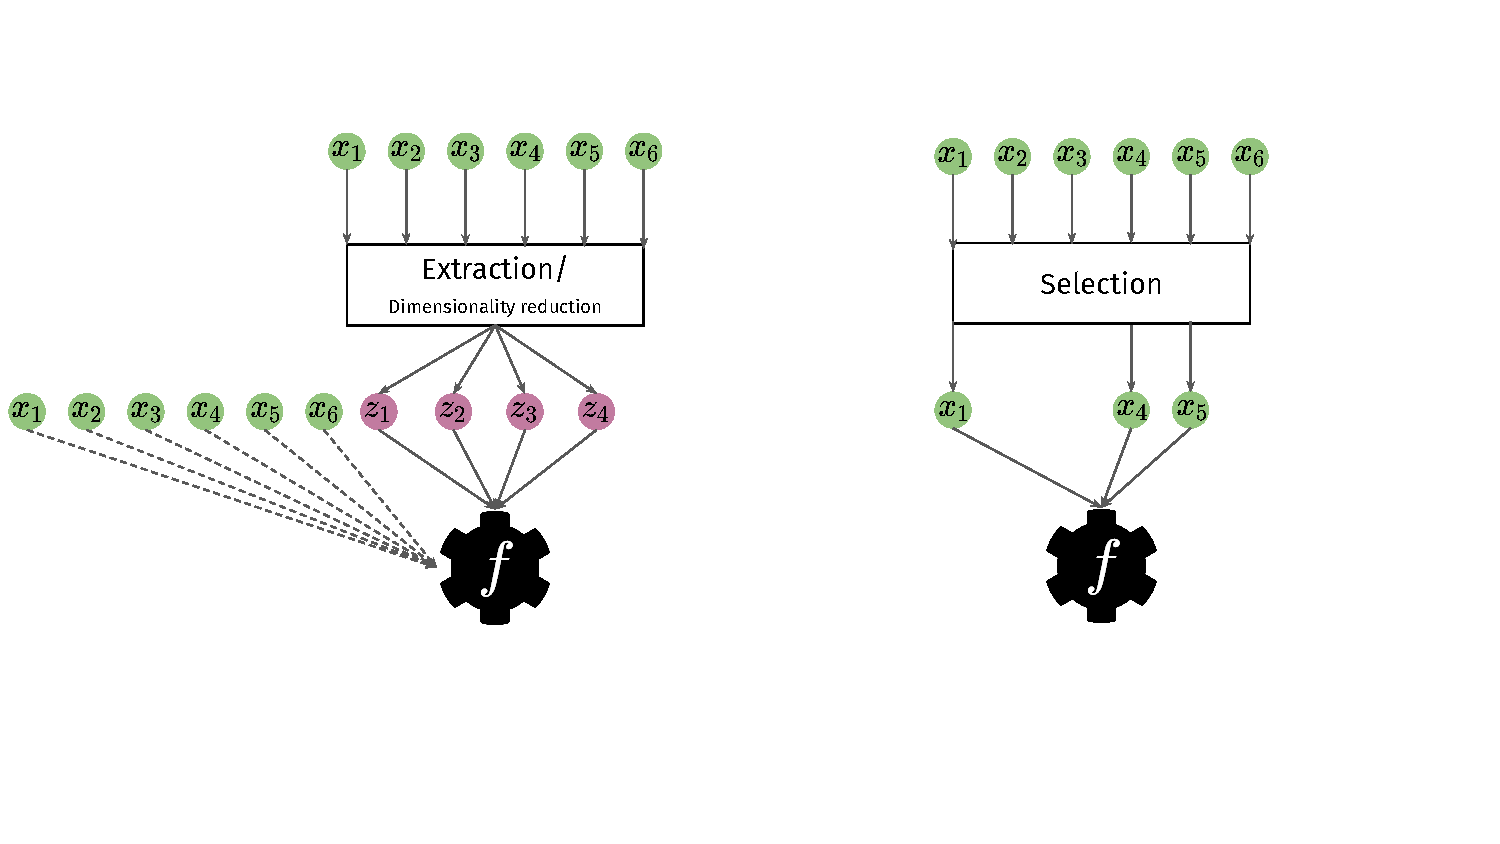
\includegraphics[width= \textwidth, trim=0 100 390 60, clip]{images/feat_extr_vs_selection.pdf}
      \end{center}
    \end{column}
  \end{columns}
    
\end{frame}


\begin{frame}{Imbalanced Classes}
  Imbalanced classes:
  \begin{itemize}
    \item over-sampling of minority class
    \item seldom: under-sampling of majority class
    \item Influence of more advanced methods (e.g.\ SMOTE) on the predictive accuracy questionable.
  \end{itemize}
\end{frame}


\section{Combined Preprocessing and Model Building: Pipelining}

\begin{frame}{Pipelining}

  Most preprocessing steps have parameters or can be switched on/off in the pipeline.

  \vspace{1em}

  \textbf{Goal:} Find optimal preprocessing parameters $\rightarrow$ HPO

  \begin{columns}
    \begin{column}{0.5\textwidth}
    \begin{itemize}
      \item Most preprocessing methods have states similar to the model of an inducer.
      \item Applying preprocessing to the whole dataset leads to overfitting.
      \item Pipeline has to be optimized as a whole: $\pcs = \pcs_{\text{pipeline}} \times \pcs_\inducer$ within the resampling procedure.
    \end{itemize}
    \end{column}%
    \begin{column}{0.5\textwidth}
      \begin{center}
        \includegraphics[page=19, width=\textwidth, trim=20 60 30 35, clip]{images/mlr3Pipelines_graphics}
      \end{center}
    \end{column}
  \end{columns}

\end{frame}

\begin{frame}{Optimizing Pipelines}

  \begin{columns}
    \begin{column}{0.6\textwidth}
      \vspace*{-0.5em}
      \begin{itemize}
        \item Introducing different choices for preprocessing.
        \item Tuning over multiple learning algorithms.
        \item[$\rightarrow$] $\pcs$ becomes hierarchical search space!
      \end{itemize}
      
      \vspace*{0.5em}

      Suitable optimizers:
      \begin{itemize}
        \item Random Search, TPE, Hyperband
        \item BO with RF surrogate
        \item Evolutionary approaches (similar to NAS)
      \end{itemize}

    \end{column}%
    \begin{column}{0.4\textwidth}
      \begin{center}
        %\includegraphics[page=7, width=\textwidth, trim=160 0 30 160, clip]{images/mlr3Pipelines_graphics}
        %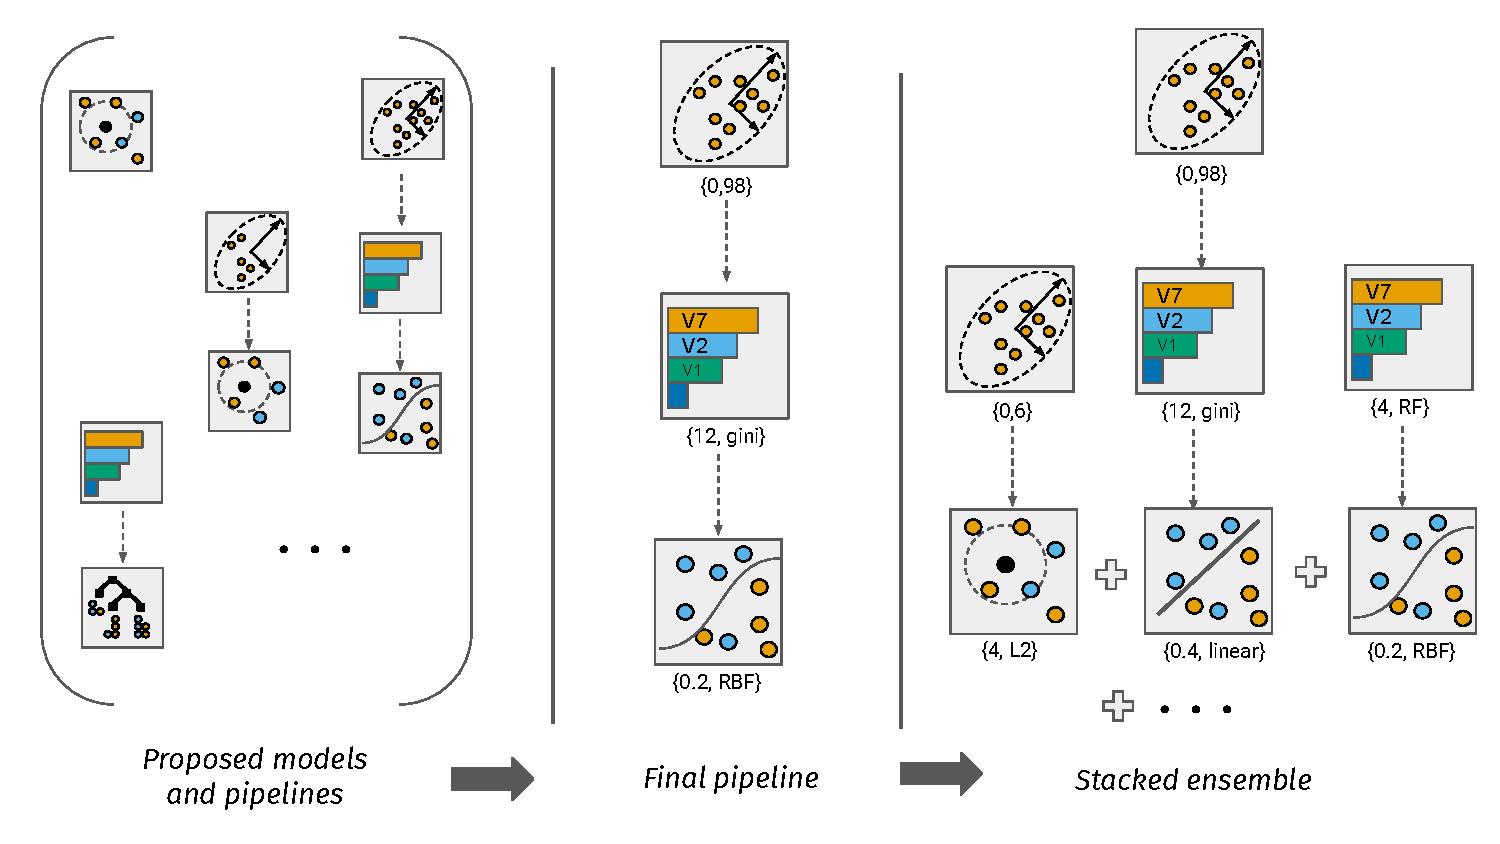
\includegraphics[width = \textwidth]{images/stacking.pdf}
        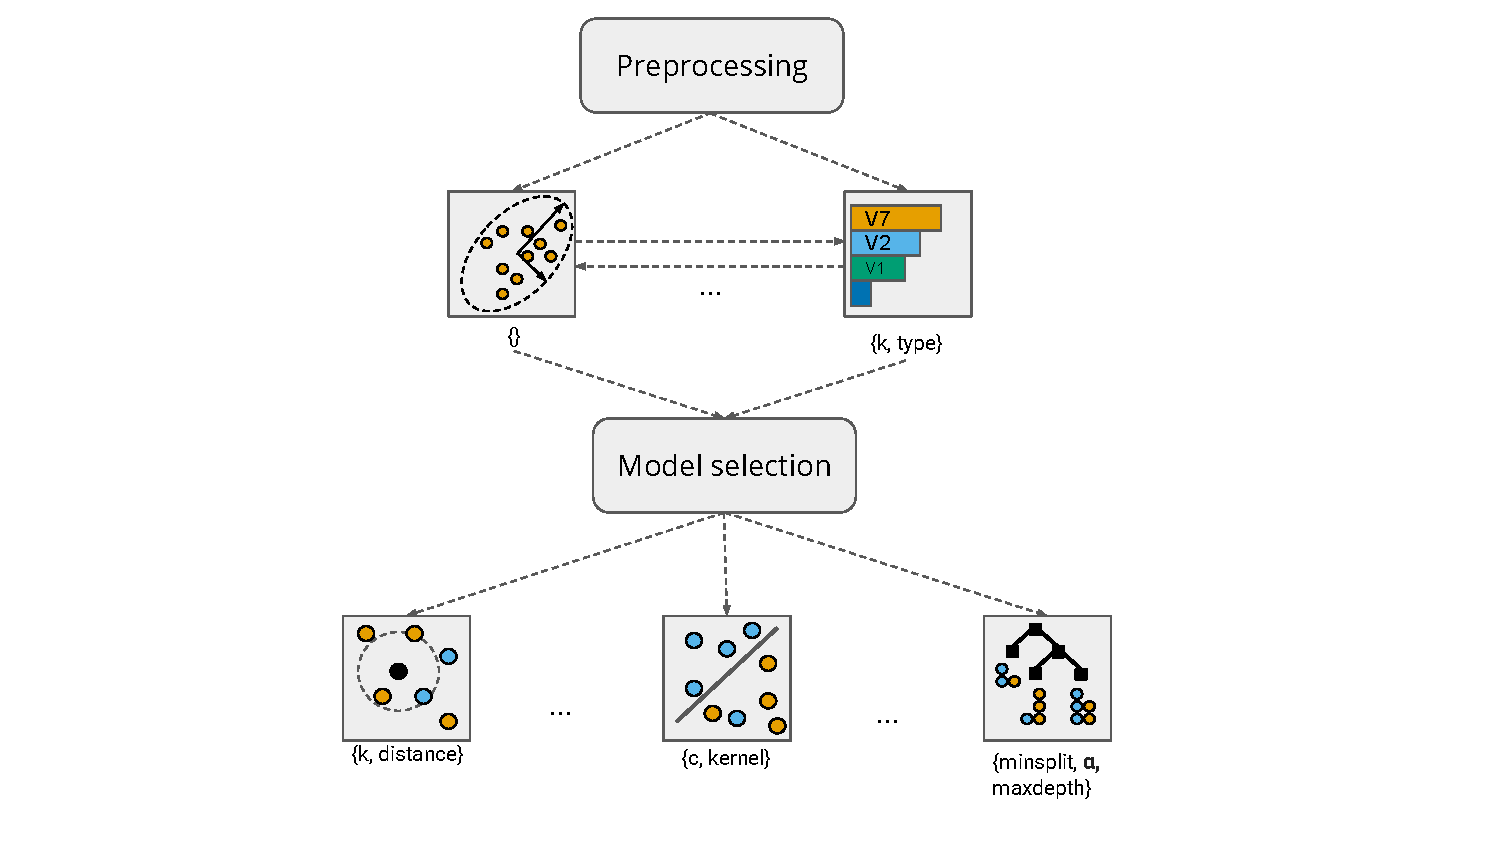
\includegraphics[width = \textwidth, trim=160 0 160 5, clip]{images/dag.pdf}
      \end{center}
    \end{column}
  \end{columns}
\end{frame}

\begin{frame}{Obtaining Final Model}

      Options:
      \begin{itemize}
        \item Choose the optimal path as linear pipeline.
        \item Build ensemble of best configurations (e.g. \lit{\href{https://www.automl.org/wp-content/uploads/2020/07/AutoML_2020_paper_61.pdf}{H2O AutoML, LeDell et al., 2020}}).
      \end{itemize}
      \begin{center}
        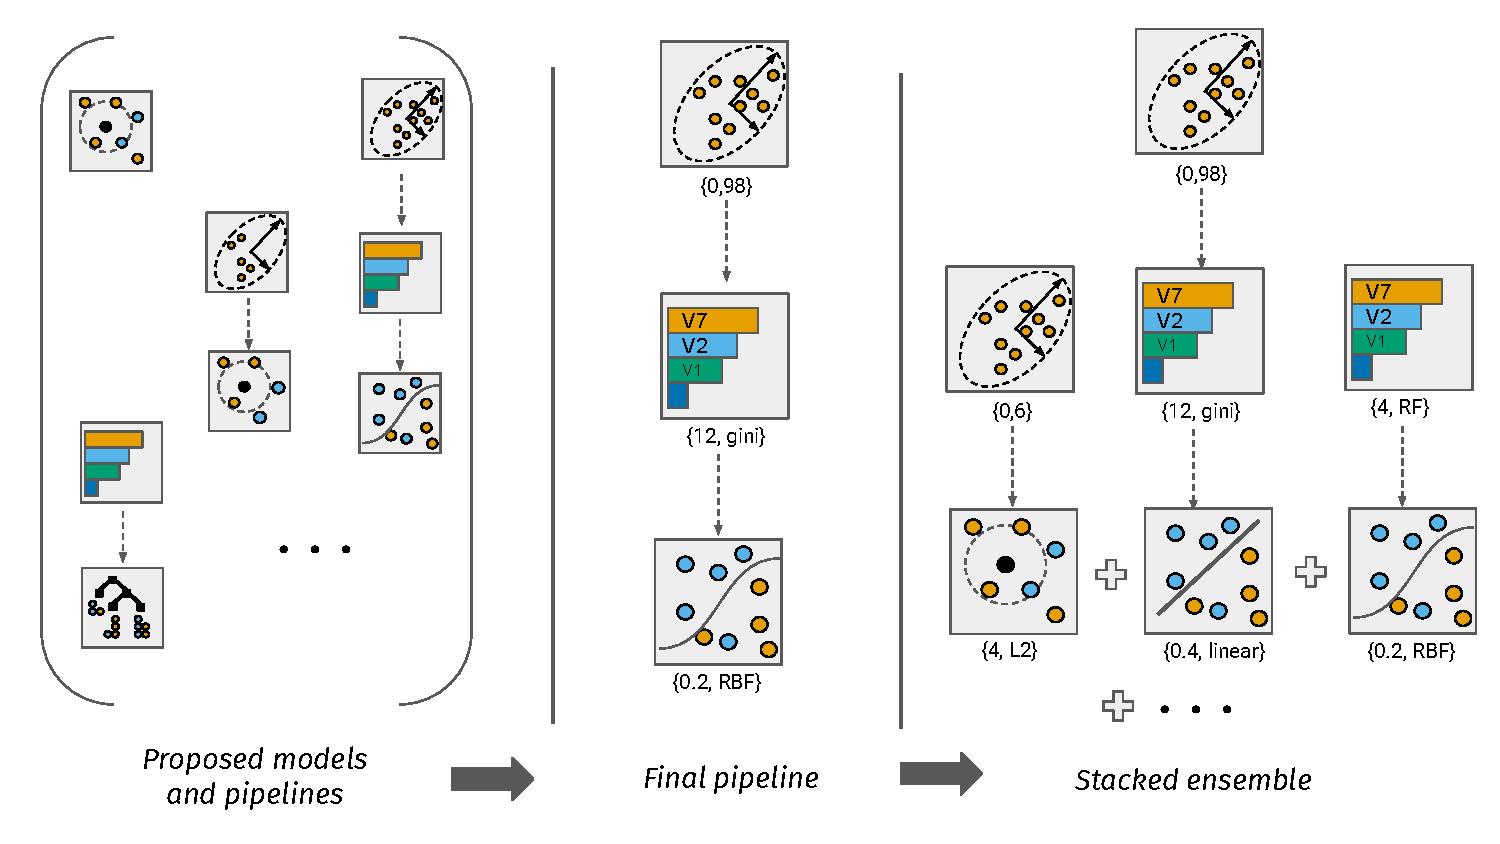
\includegraphics[width = 0.66\textwidth]{images/stacking.pdf}
      \end{center}
    
\end{frame}

% \begin{frame}[containsverbatim,allowframebreaks]{Software}

% \begin{itemize}
%   \item DataRobot (comercial, gui)
%   \item H20.ai (comercial but open source, r, python)
%   \item TPOT, Tree-based Pipeline Optimization Tool  (2016-cont, open source, evolutionary approach) % show plot https://github.com/EpistasisLab/tpot
%   \item AutoWEKA (2016, open source)
%   \item mlr3automl (2020, prelim)
%   \item Hyperopt-Sklearn (2014-cont) Only HPO
%   \item Auto-Sklearn (2.0) (2015-cont) BO, ensembles, meta-learning
% \end{itemize}

% \end{frame}



\end{document}
